\def\mySecNum{10.4}
\mySection{\mySecNum~Put options}
%-------------- start slide -------------------------------%{{{ 1
\begin{frame}[fragile,t]
\begin{center}
	We compute put option prices using the same stock price tree and in almost the same way as call option prices
	\bigskip

	The only difference with a European put option occurs at expiration

	Instead of computing the price as
	\begin{align*}
		\textcolor{magenta}{\max\left(0,S-K\right)}
	\end{align*}
	we use
	\begin{align*}
		\textcolor{cyan}{\max\left(0,K-S\right)}
	\end{align*}
\end{center}
\end{frame}
%-------------- end slide -------------------------------%}}}
%-------------- start slide -------------------------------%{{{ 1
\begin{frame}[fragile,t]
\begin{center}
	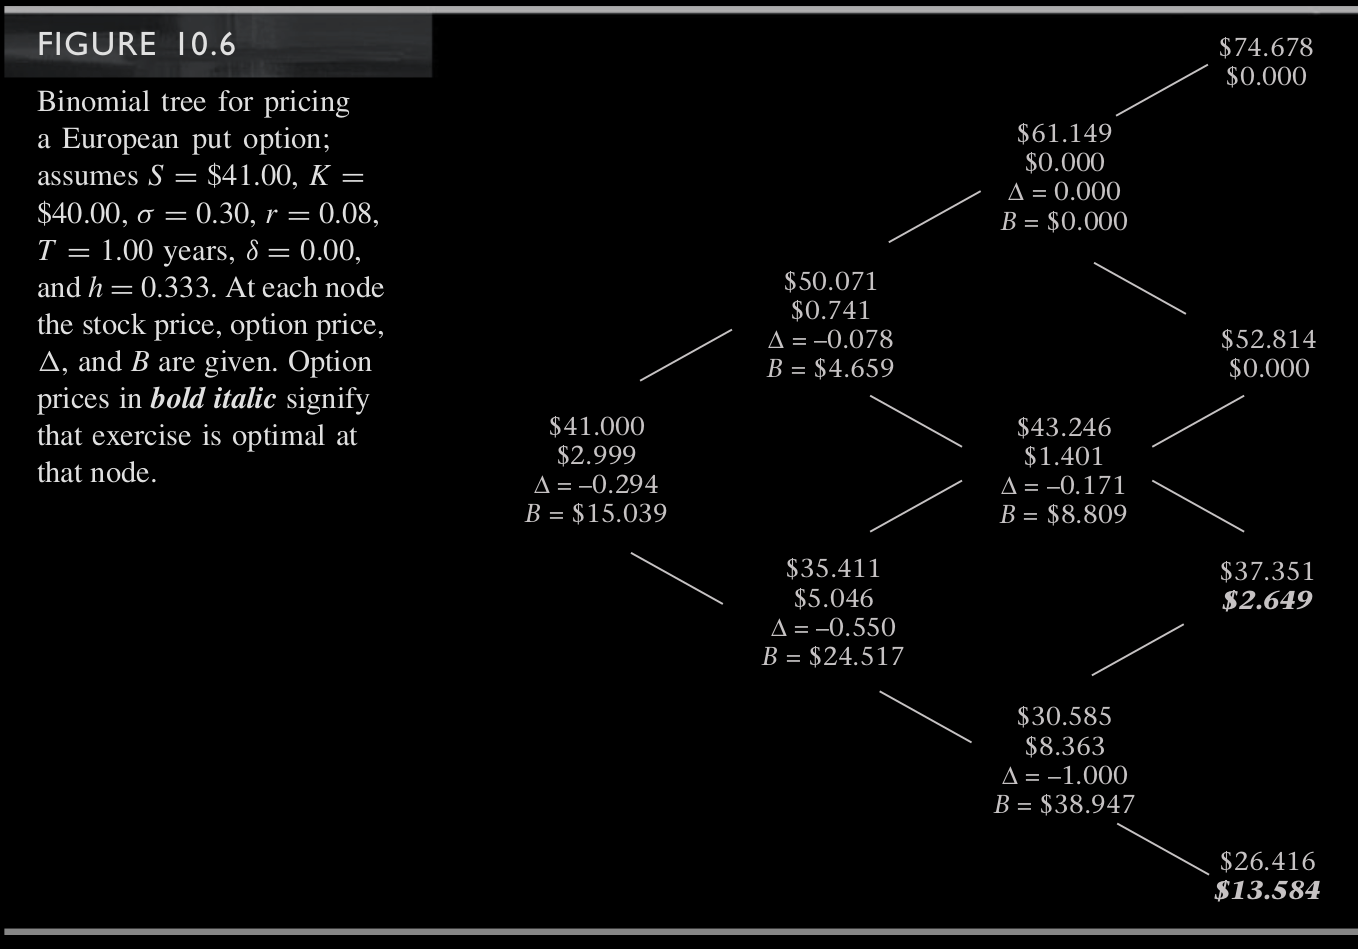
\includegraphics[scale=0.25]{figs/Figure-10-6.png}
\end{center}
\end{frame}
%-------------- end slide -------------------------------%}}}
